\documentclass[a4paper, 11pt]{article}
\usepackage{graphicx}

\title{%
\vspace{-2.5cm}
\textbf{Nintendo Entertainment System Emulator}\\
User Personas and Use Cases
}
\date{\today}
\author{Kajetan Lach}

\begin{document}

\maketitle

\section{Introduction}
This document contains \textbf{profiles of primary user groups} potentially interested in using our Nintendo Entertainment System Emulator, identifying their motivations, goals and use cases.

\section{Alex - Computer Science Student and Aspiring Developer}
Alex is a 21-year-old undergraduate \textbf{Computer Science student}. Exposed to computers from an early age, he developed a natural interest in programming, which aligns with his lifelong passion for computer games, problem-solving and engineering mindset.

\begin{figure}[h]
    \centering
    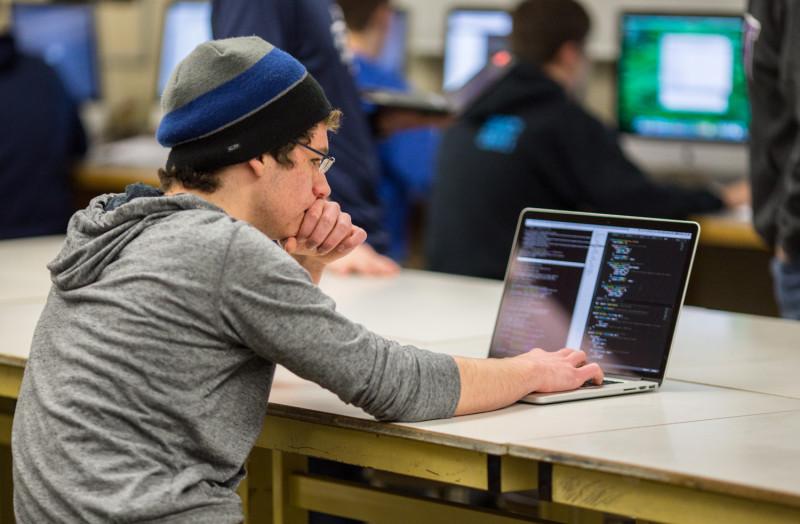
\includegraphics[width=0.7\textwidth]{student-coding.jpg}
\end{figure}

\subsection{User Goals and Motivations}
Alex's main motivation to use our NES emulator is to \textbf{gain practical experience in computer architecture and low-level programming} while \textbf{staying engaged} with retro games and well-known franchises. He aims to develop a solid understanding of CPU instructions, memory management and system emulation. Alex plans to use the emulator's tools and documentation as \textbf{study aids for coursework and personal projects}. He might pick emulation for his next free-time project's theme.

\subsection{Product Value for the User}
Our product offers Alex a \textbf{clean, well-organized and open codebase}, along with \textbf{detailed documentation, debugging tools and tutorials on emulator development}. The program's open structure allows Alex to step through code execution in detail, helping him deepen his understanding of system architecture and memory management.

\subsection{Use Case}
Alex wants to explore CPU emulation for studying purposes. He opens the emulator, loads a simple ROM and observes program execution. He follows instruction cycles, monitors memory usage and check registers content. Using the documentation, he cross-references CPU behavior to understand how the emulator translates instructions. In the process, \textbf{he gains real-time insights into CPU architecture and operation cycles, directly linking this knowledge to his coursework}.

\section{Alice - Computer Science Lecturer or Teacher}
Alice is a 45-year-old \textbf{university lecturer in computer science}, teaching introductory courses on programming, computer architecture, and embedded systems.

\begin{figure}[h]
    \centering
    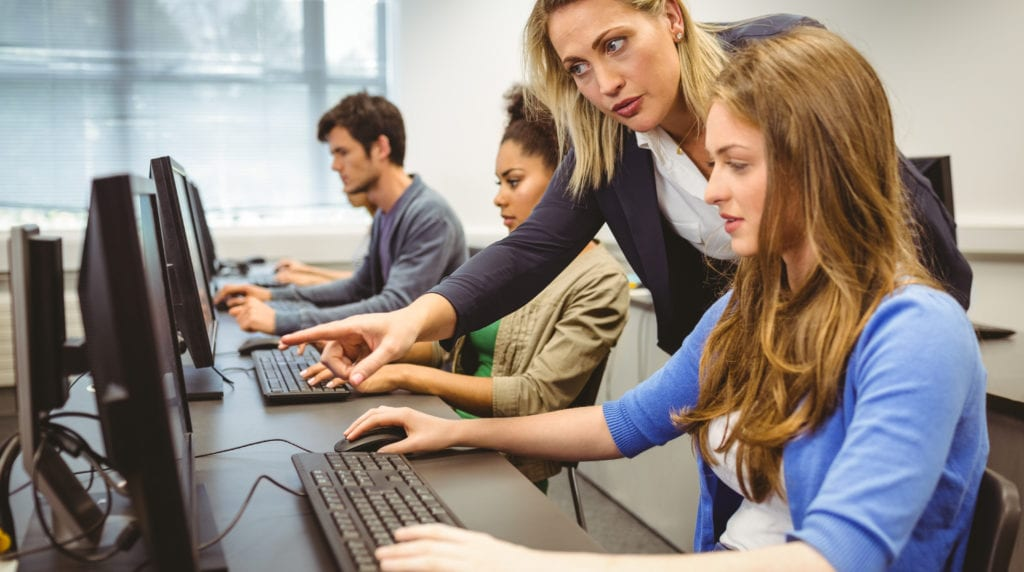
\includegraphics[width=0.7\textwidth]{teacher.jpg}
\end{figure}

\subsection{User Goals and Motivations}
Alice is passionate about teaching and \textbf{seeks practical resources to keep students engaged and make technical concepts easier for them to grasp}. She believes that with hands-on experience and demonstration, even the toughest concepts can be understood.

\subsection{Product Value for the User}
Our emulator provides Alice with an \textbf{effective educational tool to demonstrate fundamental computing concepts and offer practical experience, all within an engaging retro games theme}. It enables her to present abstract concepts in an accessible, visual format that makes technical learning memorable.

\subsection{Use Case}
Alice provides students with an \textbf{assignment to load a simple NES program and analyze memory usage}. She requires them to use the emulator's debugging tools to observe and document how the program manages memory. Afterward, she collects and reviews students' finding, using their analyses to discuss course topics.

\section{Bob - Casual Gamer}
Bob is a 41-year-old \textbf{gaming enthusiast} who has been passionate about video games for as long as he can remember, creating countless memories with his favourite titles. Now, as a father, he shares this passion with his 8-year-old son.

\begin{figure}[h]
    \centering
    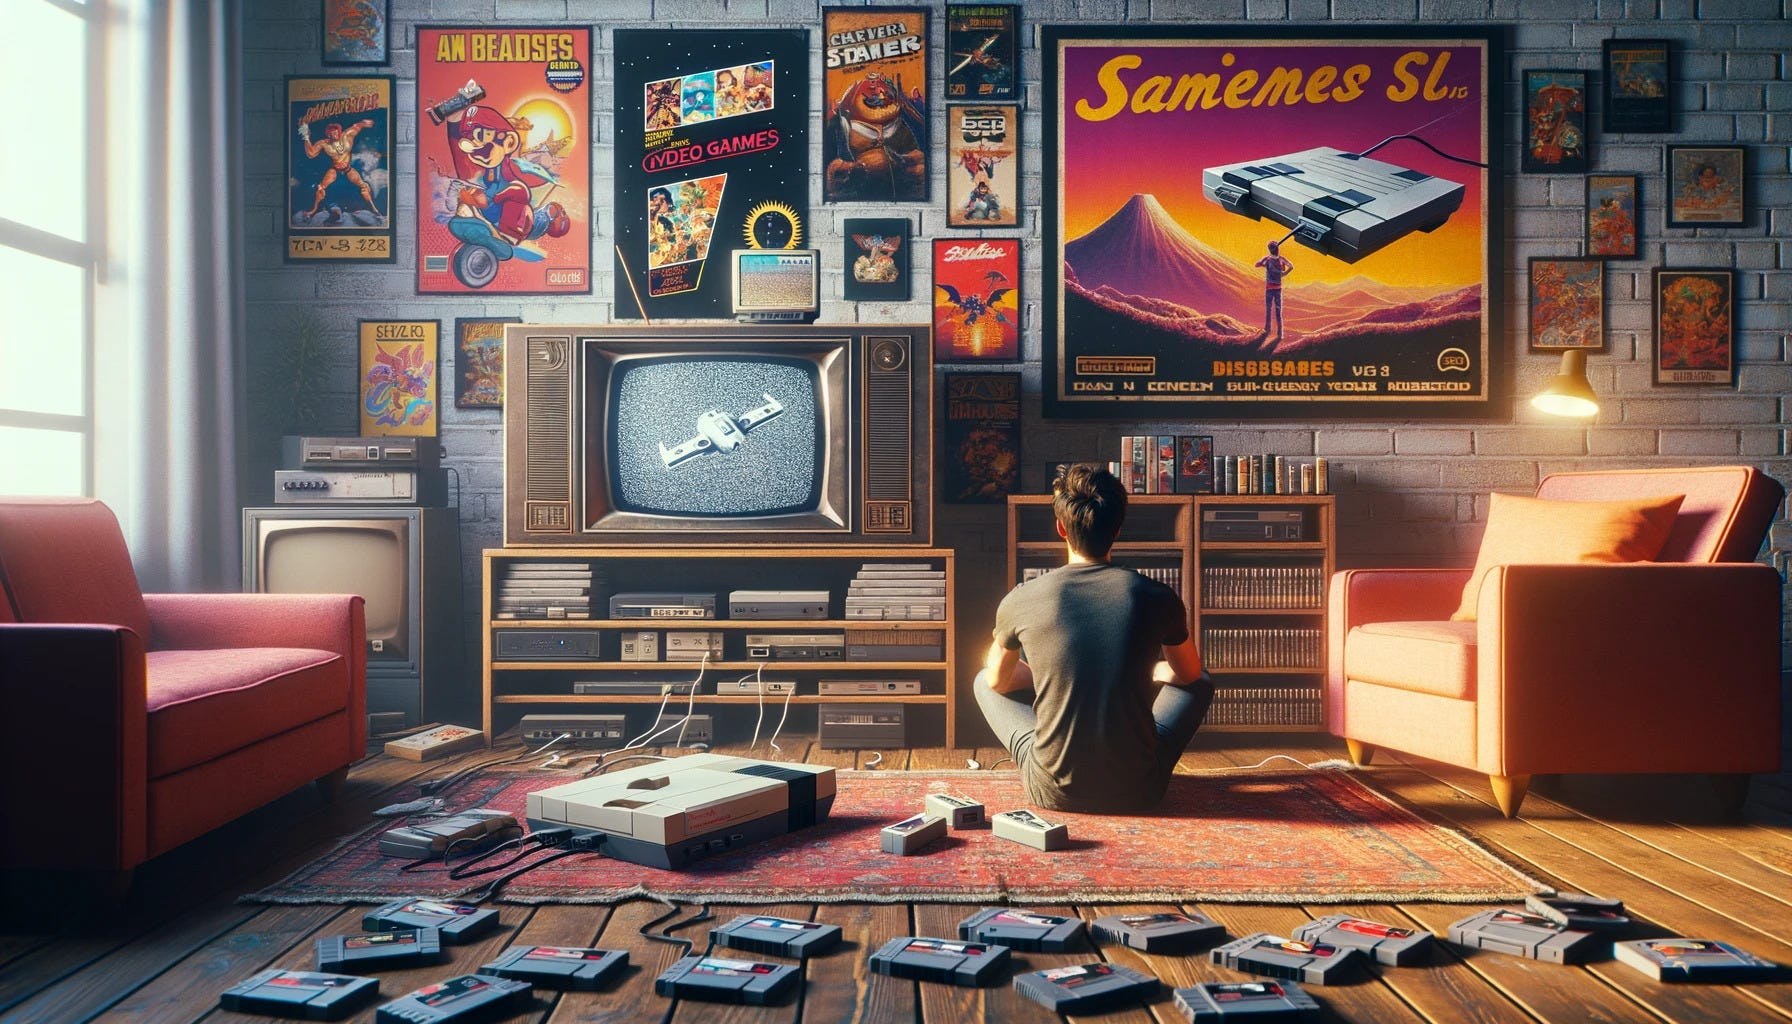
\includegraphics[width=0.7\textwidth]{vintage-console.jpg}
\end{figure}

\subsection{User Goals and Motivations}
Bob wants to \textbf{revisit nostalgic games} that are hard to access without emulation. Also, he hopes to \textbf{share these childhood memories with his son}, showing him how games used to look and feel. Emulation allows Bob to appreciate how games were once created, giving him insight into the technological changes since he was his son's age.
\subsection{Product Value for the User}
The NES Emulator offers a \textbf{convenient and authentic way to revisit games Bob grew up with}, without requiring any additional hardware or complex setup. Bob can share his memories with his son, introducing him to the classics. For Bob, who enjoys exploring the technical side of things, \textbf{the emulator's debugging tools and documentation} allow him to dive into game mechanics and satisfy his curiosity about game design. Since video games are primarily a source of entertainment for Bob, the emulator gives him a \textbf{reliable and stable environment} to play in.

\subsection{Use Case}
Bob loads a ROM in debugging mode to show his son how games used to store important information, like health or points. He identifies the register where the game stores the player's health and makes slight adjustments to its contents, demonstrating to his curious son how this changes the game's behavior. \textbf{Together, they explore how video games looked like when Bob was his son's age, and he enjoys revisiting the titles he grew up with}.

\end{document}